\documentclass[useAMS,usenatbib]{mn2e}
\usepackage{graphicx}
\usepackage{url}

%\usepackage{tikz}
\newcommand{\aap}{Astron. Astrophys.}
\newcommand{\aj}{Astron. J.}
\newcommand{\ao}{Appl. Opt.}
\newcommand{\apj}{Astrophys. J.}
\newcommand{\apjl}{Astrophys. J. Lett.}
\newcommand{\apjs}{Astrophys. J. Suppl.}
\newcommand{\mnras}{Mon. Not. Roy. Ast. Soc.}
\newcommand{\nat}{Nature}
\newcommand{\pasa}{Publ. Ast. Soc. Aust.}
\newcommand{\pasp}{Publ. Ast. Soc. Pac.}
\newcommand{\prl}{Phys. Rev. Lett.}
\newcommand{\prd}{Phys. Rev. D}
\newcommand{\msun}{\mathrm{M}_\odot}

\title[Inpainting]{Inpainting of Galaxy Redshift Surveys}
\author[Antolini, Caiazzo \& Heyl]{Elisa Antolini$^{1}$, Ilaria Caiazzo$^{2}$, Jeremy S. Heyl$\thanks{Email:
    heyl@phas.ubc.ca; Canada Research Chair}^{2}$ \\
  $^{1}$Dipartimento di Fisica e Geologia, Universit\`a degli Studi di Perugia, I-06123 Perugia, Italia \\
  $^{2}$Department of Physics and Astronomy, University of British
  Columbia, 6224 Agricultural Road, Vancouver, BC V6T 1Z1, Canada\\
}
\begin{document}
\date{Accepted ---. Received ---; in original form ---}

\pagerange{\pageref{firstpage}--\pageref{lastpage}} \pubyear{2016}

\maketitle

\label{firstpage}

\begin{abstract}
\end{abstract}

\section{The Tecnhique}
\label{sec:tecnhique}
The technique is straightforward to describe and to implement, and we
will outline it below.  Let the map be given by $a(\Omega)$ and the
mask by $m(\Omega)$ where $m(\Omega)=1$ where the underlying galaxies
are visible.
\begin{enumerate}
\item
  Set an initial guess for the underlying map.
\begin{equation}
  y_1(\Omega) = \frac{\left \langle  m(\Omega) a(\Omega)  \right \rangle}{\left \langle m(\Omega) \right \rangle }
    \label{eq:2}
\end{equation}
\item
  Calculate the residual of the current guess
  \begin{equation}
    r_t(\Omega) =  m(\Omega) a(\Omega) - y_t(\Omega)
    \label{eq:3}
  \end{equation}
\item
  Expand the sum of the residuals in the unmasked region and the current guess
  in spherical harmonics.
  \begin{equation}
    A_{lm,t} = \int d\Omega Y^*_{lm} \left [ m(\Omega) r_t(\Omega) + y_t(\Omega) \right ]
    \label{eq:4}
  \end{equation}
\item
  Keep only the components with the largest amplitudes and set the
  amplitudes smaller than the threshold ($\lambda_t$) to zero.
\item
  Calculate the new guess from the largest components
  \begin{equation}
    y_{t+1}(\Omega) = \sum_{|A_{lm,t}| > \lambda_t} A_{lm,t} Y_{lm}(\Omega).
    \label{eq:5}
  \end{equation}
\item
  Decrease the threshold $\lambda_t$ and repeat from step (ii) until the stopping criterion
  is reached.
\end{enumerate}
There is of course some art in choosing the size of the underlying
basis, the thresholds and the stopping criterion.  Here we expand the
galaxy map to $l_\mathrm{max}=m_\mathrm{max}=64$, so there are a total
of 2,145 components.  The threshold is set to keep a given fraction of
the components at each step.  The fraction increases from $10^{-3.5}$
to $10^{-0.5}$ over 200 iterations, so the initial representations use
just a few components and the number of components increases to about
680 at the final iteration, so over two thirds of the spherical
harmonic components are set to zero in the final map.

From the iterative procedure above it is apparent that the value of
the guess within the masked region (where $m(\Omega)=0$) does not
contribute to the residual and does not influence the solution.
However, the spherical harmonics that contribute to the data near the
edge of the mask do influence the guess within the masked region.

fake test gives R=0.70

\section{Tests}
\label{sec:tests}


\subsection{Simulated Maps}
\label{sec:simulated-maps}

To understand the effectiveness of these techniques we simulate galaxy
sky maps with the Galactic plane hidden and cross-correlate the
restructed galaxy maps with the original simulated map.  For make the
simulation as realistic as possible we use the angular power spectrum
of the observed galaxy map from 2MASS to construct the test maps.
These simulated maps by design have the same angular power spectrum as
the real 2MASS data including the zone of avoidance but different
phases, so they don't exhibit a zone of avoidance and they lack the
potential higher order correlations that the data may exhibit.
Fig.~\ref{fig:galmap} depicts a particular example of this technique.
We used the angular power spectrum of the upper panel to create one
hundred independent maps with the same power spectrum; one of these is
depicted in the middle panel of the figure.  We masked the Galactic
plane and used the infilling techinique to fill in the region.  The
lower panel depicts the difference between in the infilled map and the
original.
\begin{figure}
  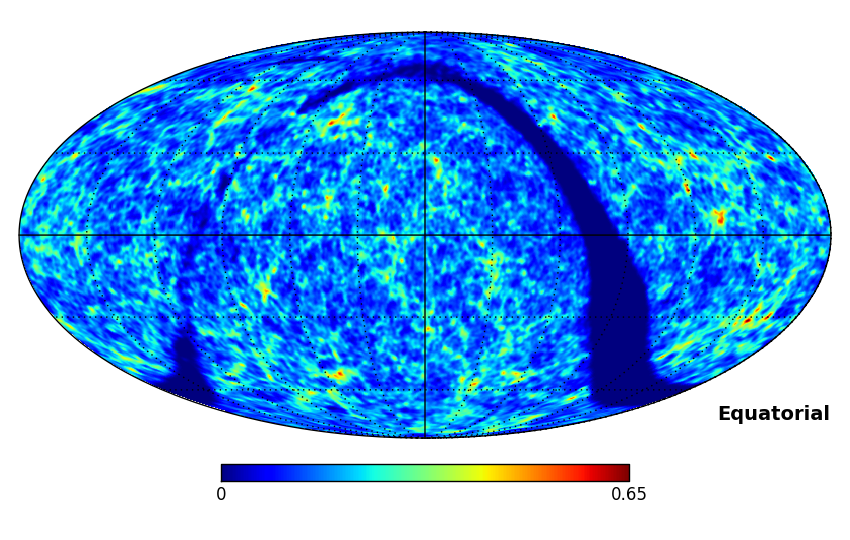
\includegraphics[width=\columnwidth]{cleantest_000/orig_map}
  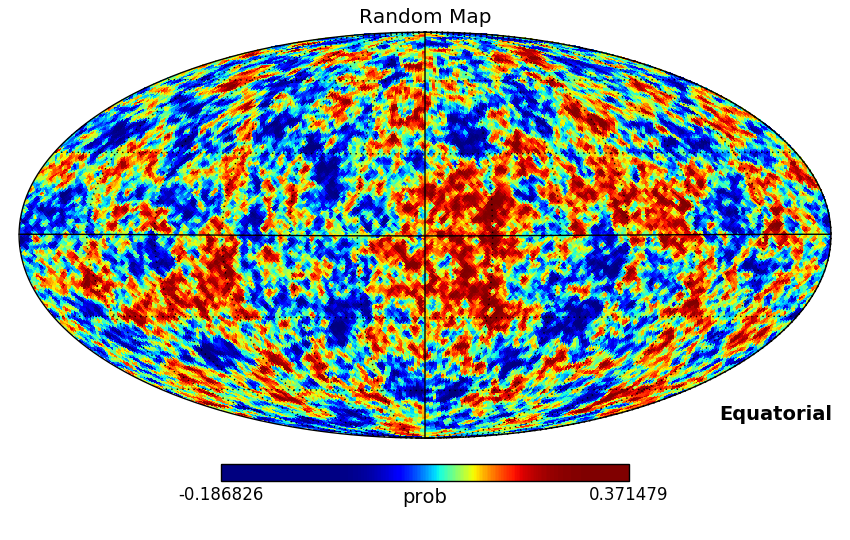
\includegraphics[width=\columnwidth]{cleantest_000/RandMap}
  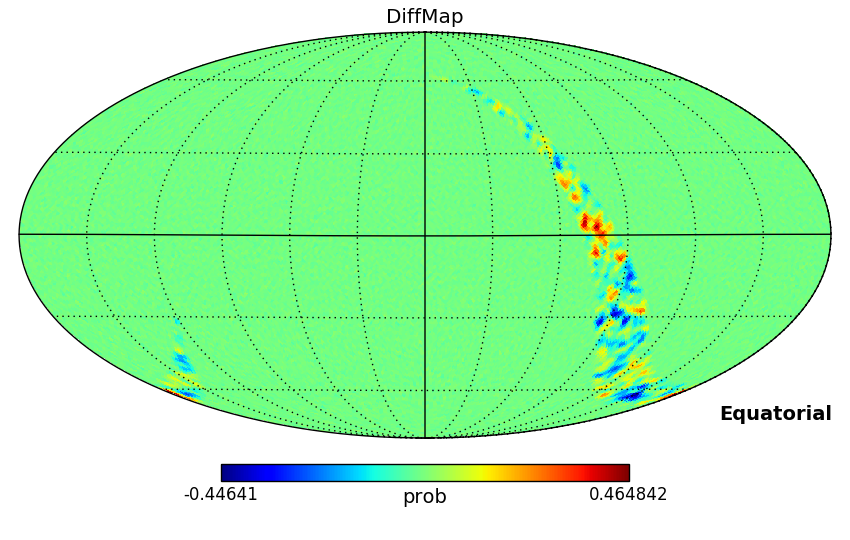
\includegraphics[width=\columnwidth]{cleantest_000/DiffMap}
  \caption{Upper: the relative surface density of galaxies in the
    2-MASS Photometric Redshift Survey with photometric redshifts
    between 0.01 and 0.1, smoothed with a Gaussian of 0.6 degrees
    (0.01 radian), the input map.  Middle: the test map constructed
    using the angular power spectrum of the map in the upper panel.
    Lower: we masked the Galactic plane of the middle panel and
    reconstructed the image using the techinque in
    \S~\ref{sec:tecnhique}.  The difference between the middle panel
    and the reconstructed map is depicted.}
  \label{fig:testmap}
\end{figure}

To make statistic sense of the agreement we calculate Pearson's
correlation coefficient ($r$) between the original data and the
infilled reproduction within the infilled region for each of the
trials and examine its cumulative distribution as depicted in
Fig.~

\begin{figure}
  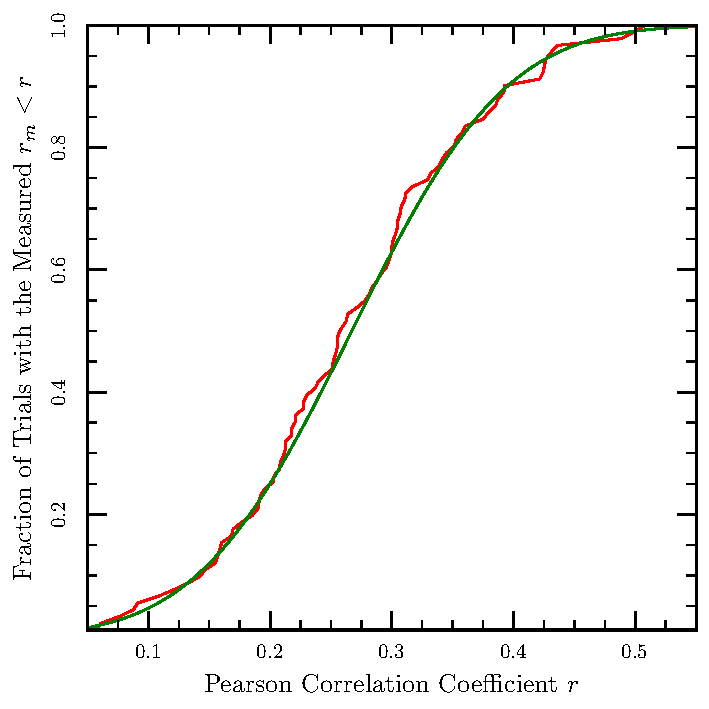
\includegraphics[width=\columnwidth]{cleantest}
  \caption{Cumulative distribution of $r$ for 100 trials of the
    infilling procedure with simulated data}
\end{figure}


\subsection{Observed Maps}

\section{Results}

\section{Discussion}


\bibliography{infill}
\bibliographystyle{apj}

\label{lastpage}


\end{document}
